%%!TEX ROOT = ../mainCZ.tex



Do modelu vstupují informace o topografii řešeného území, informace o typech půd a využití území a o jejich prostorovém rozmístění, informace o srážce, případně o geometrii dočasné hydrografické sítě.
Tato data jsou zadávána ve třech formátech: rastrovém, vektorovém a textovém. 
% Do modelu vstupují informace o topografii řešeného území, informace o typech půd a vegetaci, informace o srážce atd. 
Základní formát vektorových dat je formát shapefile. Tento vektorový formát byl vytvořen firmou ESRI, ale je zpracovatelný i jinými GIS softwary. Parametry modelu jsou uloženy v atributové tabulce pod specifickým názvem pole. 
% Shapefile popisuje prvky jako body, linie nebo polygony. Každý prvek má obvykle nějaký atribut, který ho popisuje jako v tomto případě jméno, či typ půdy. 
V následujícím textu jsou popsány náležitosti vstupních dat. 
% 
% Model pracuje s následujícími vstupy
Přehled vstupů do modelu je ukázán v tabulce~\ref{tab:vstupy}.


% 

% 
\begin{sidewaystable}
% \begin{table}[]
\centering
\caption{Tabulka s přehledem vstulních dat modelu}
\label{tab:vstupy}
\small{
% \begin{tabular}{p{4cm}lp{2cm}p{5cm}}
\begin{tabular}{p{0.30\textwidth}lp{0.10\textwidth}p{0.30\textwidth}l}
\hline \hline
Název                              & Typ dat                       & Povinný / volitelný & Poznámka                                                                                      & Více v kapitole                                                 \\ \hline 
digitální model terénu             & raster                        & Povinný           & Touto vrstvou se řídí i prostorová diskretizace.                                                 & \ref{sec:vstupdmt}                                           \\ 
prostorové rozložení půd           & vektor - polygony             & Povinný           & V atributové tabulce identifikátor typu půdy.                                               & \ref{sec:vstuppuda}                                          \\ 
prostorové rozložení využití území & vektor- polygony              & Povinný           & V atributové tabulce identifikátor využití území.                                           & \ref{sec:vstupvegetace} a \ref{sec:upravatabulkyparametru}   \\ 
srážková data                      & .txt soubor                   & Povinný           & Kumulativně zadaná srážka.                                                                       & \ref{sec:vstupsrazka}                                        \\ 
maximální časový krok              & reálné číslo                  & Povinný           & Model mění délku časového podle odtokových podmínek; doporučuje se 30 - 60 sekund.               & \ref{sec:vstupkrok}                                          \\ 
výstupní adrešář                   & text                          & Povinný           & Adresář k uložení výsledků (při spuštění výpočtu se obsah adresáře vymaže!).                            & \ref{sec:vstupadresar}                                       \\ 
bodové výstupy hydrogramů          & vektor - body                 & Volitelný         & Body pro výpis výsledků.                                                                   & \ref{sec:vstupbody}                                          \\ 
% typ výpočtu                        & text                          & Povinný           & Uživatel má na výběr: pouze plošní odtok, plošný i rýhový odtok, plošný, rýhový odtok i odtok hydrografickou sítí               & \ref{sec:vstupryhovy}          \\ 
% volba výcesměrného odtoku          & logická proměnná              & Povinný           & Jednosměrný (výchozí)  nebo vícesměnný odtok                                                           & \ref{sec:vstupvicesmerny}      \\ 
paramtry půdy a využití území           & tabulka                       & Povinný           & Tabulka parametrů půdy a využití území. Názvy sloupců mají definované označení. Hodnoty se spojí s vektorovými vrstvami.            & \ref{sec:upravatabulkyparametru}\\ 
hydrografická síť                  & vektor - linie                & Volitelný         & Prostorové rozložení hydrografické sítě. Atributová tabulka obsahuje identifikátor tvaru jednotlivých úseků.        & \ref{sec:vodnitoky}             \\ 
parametry úseků hydrografické sítě       & tabulka                       & Volitelný         & Tabulka parametrů jednotlivých úseků hydrografické sítě.                                                                        &  \ref{sec:vodnitoky}     \\ 
volba arcgis výstupů               & logická proměnná              & Povinný           & Výchozí formát výstupních rastrů je proprietární formát ERSI. Uživatel může zvolit textový formát ASCII.                       & --- \\ \hline \hline
\end{tabular}
}
% \end{table}
\end{sidewaystable}
% \begin{itemize} \itemsep 0pt
% \item digitální model terénu
% \item shapefile půd
% \item shapefile využití území
% \item srážkový soubor
% \item časový krok výpočtu a celková doba simulace
% \item výstupní adresář
% \item bodová vrstva pro generování hydrogramů
% \item výstupní adresář
% \item typ výpočtu
% \item volba výcesměrného odtoku
% \item tabulka půd a vegetace a kód pro připojení
% \item shapefile hydrografické sítě
% \item tabulka vodních toků a kód pro připojení
% \item volitelné formy výstupů
% \end{itemize}

% 
% \pozn{
% \textbf{Nutno dodělat}
% \begin{itemize} \itemsep 0pt
% \item upravit podle aktuálního stavu
% \item upravit a zjednosušit tuto kapitolu
% \item propojit s tabulkama co jsou jinde v textu
% \item vložit sem tabulky parametrů výpočtu pokud nejsou jinde
% \end{itemize}
% }
% 
% 
% 
% 
% 
% 









\subsection{Digitální model terénu} \label{sec:vstupdmt} 

Rastr digitálního modelu terénu DMT, či anglicky DTM (Digital Terrain Model) reprezentuje souvislou morfologii určité části Země. DMT rastr je složen z jednotlivých buněk obsahující informaci o elevaci terénu.  Velikost buněk se liší v závislosti na velikosti zobrazovaného území. Pro účely modelu \smod by minimální velikost buněk měla být 2 metry, optimum je však 5 metrů a více. Model byl testován na rastrech o velikosti od několika málo do stovek tisíc buněk. DMT jednoho z testovacích povodí, povodí Nučice, obsahuje přes 125 tisíc buněk při velikosti buňky 5 $m$. Příklad DMT dalšího testovacího povodí Býkovice je ukázán na obrázku~\ref{fig:dmt}.


% 
% \begin{figure}
%   \centering
%   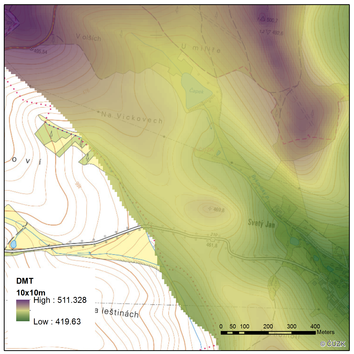
\includegraphics[width=0.5\textwidth]{./img/DMT_byk.png}
%   \caption{Výřez digitálního modelu terénu povodí Býkovice}
%   \label{fig:bykovicedmt}
% \end{figure}

 
 
 
 
 
 
 
 
 
 
 
 
 
 
 
 
 
 
 
\subsection{Půdní data} \label{sec:vstuppuda}


Vstupem do modelu je vektorová vrstva s vymezením jednotlivých půd.

Z hlediska půdních dat jsou obecně v ČR v rozumném měřítku podrobnosti k dispozici několik datových zdrojů. prvním je syntetická půdní mapa v měřítku 1:250 000 (KPP250), která vychází z komplexního průzkumu půd, tento datový podklad byl odvozen z předešlé tištěné mapy, čemuž také odpovídá měřítko podrobnosti dat. Po rozdělení půdního fondu na lesní a zemědělskou půdu jsou dalšími zdroji oddělené databáze pro tyto dvě skupiny. Na zemědělské půdě je dostupná půdní typologie (ve formě kódu BPEJ, resp. HPJ),  v současné době uvolněná k využití na portálu SPÚ. Prakticky neexistuje vhodný převodní klíč mezi hodnotami BPEJ a parametry infiltračních rovnic. Půdní druhy vyjadřující zrnitost ornice a podorničí podle Novákovy klasifikace je možné získat na VÚMOP v.v.i., dle aktuálního ceníku jako vektorovou vrstvu ve formátu shp. Dále jsou na portálu kpp.vumop.cz dostupné informace o konkrétních půdních sondách průzkumu KPP (kpp.vumop.cz).

V případě lesních půd, lesnické typologie a informací o půdních charakteristikách je dostupnost dat omezená. Veřejně dostupné jsou kódy lesnické typologie, ale metodika pro převod kódované informace na hydrologické vlastnosti půd (Macků, 2012) není dohledatelná. Hloubka lesních půd, zrnitostní složení a některé další charakteristiky jsou k dispozici na Ústavu pro hospodářskou úpravu lesů (ÚHUL), ale jejich poskytnutí vyžaduje součinnost s uvedeným úřadem. 

V případě využití modelu jsou klíčovým vstupem hydraulické charakteristiky půd, zejména nasycená hydraulická vodivost \acs{Ks}. Tato veličina je závislá na řadě půdních charakteristik, nejčastěji je vztahována k jejímu zrnitostnímu složení. Regionalizované informace o zrnitosti půd lze v ČR získat z výše jmenovaných datových zdrojů. 

Kromě dostupnosti prostorových dat vstupuje další komplikace v podobě nesouladu v klasifikaci půd na lesní půdě (USDA) a zemědělské (Novákova klasifikace). Syntéza těchto dat není triviální.
Průměrné hodnoty \acs{Ks} pro jednotlivé zrnitostní třídy, tzv. pedotransferové funkce, jsou odvozené z rozsáhlých půdních databází, které lze nalézt zejména v zahraniční literatuře \citep{wosten1999, toth2015}. V českých podmínkách je k dispozici, počtem analyzovaných vzorků značně omezená, databáze HYPRES-CZ \citep{mihalikova2013}. Obecně se však jedná o velmi variabilní data. Vzhledem k enormnímu rozptylu hodnot je pro snížení nejistot v hydrologickém modelování velmi žádoucí zajistit alespoň základní půdní rozbor v řešené lokalitě.


Obrázek~\ref{fig:puda} ukazuje výřez připravené vrstvy. Pro určení charakteristik je nutné, aby atributová tabulka dané vrstvy obsahoval identifikátor půdního typu. Identifikátor odkazuje na půdní charakteristiky, které jsou ale uložené v samostatné tabulce (viz níže). Mezi půdní charakteristiky a parametry používané modelem patří: \acs{HyVod} - \acl{HyVod}; \acs{Sorb} - \acl{Sorb}; \acs{n} - \acl{n}, \acs{b} - \acl{b}, \acs{X} - \acl{X} a  \acs{Y} - \acl{Y}. Hodnoty těchto parametrů lze převzít z tabulky~\ref{tab:kriticke} v příloze~\ref{sec:priloha}. Fyzikální význam těchto parametrů a jejich implementace v modelu jsou popsány v části~\ref{cast:1} toho manuálu. 





 
 
 
 
 
 
 
 
 
 
\subsection{Data využití území} \label{sec:vstupvegetace}
Obdobně jako u půdních dat je vstupem vektorový shapefile popisující využití území.

Data o využití území jsou dostupné jak ve vektorové, tak rastrové podobě. Na stránkách MŽP je po registraci zdarma dostupná vrstva CORINE LandCover. Ve větším detailu je možné data o povrchu odvodit z databáze ZABAGED. Z vrstev je možné získat informace o plochách, liniových prvcích, cestní síti, vodních tocích. Využití území je možné na zemědělské půdě zpřesnit na základě dat LPIS. Převod liniových prvků na plošné je vhodné jen u prvků šířky srovnatelné se zvoleným rozlišením DMT, např. u dálnic a silnic první třídy. Rozumnou volbou podrobnosti účely hydrologického modelování je spojení vstupních vrstev do přiměřeného množství kategorií. Vhodné členění může být například:  
\begin{itemize} \itemsep -3pt
  \item orná půda,
  \item travní porosty,
  \item ostatní zeleň,
  \item vodní plochy,
  \item sady,
  \item křovinaté porosty,
  \item lesní porosty,
  \item antropogenní a zpevněné plochy,
  \item zahrady.
\end{itemize}
V kategorii zpevněných ploch jsou zařazeny jak oblasti zástavby, tak zpevněné komunikace s přiměřeným rozšířením podle kategorie silnice. 
\pozn{????Orientační hodnoty poměrné plochy listové (Ppl), potenciální intercepce (Pi), povrchové drsnosti a retence jsou uvedeny v příloze.
}

Shapefile popisující využití území je ukázán na obrázku~\ref{fig:LU}. Obdobně jako u půd v předchozí sekci je třeba atributovou tabulku tohoto shapefilu doplnit o identifikátor daného využití území. Tento identifikátor odkazuje na charakteristiky daného povrchu definované ve zvláštní tabulce (popsáno v sekci~\ref{sec:upravatabulkyparametru}). Parametry související s využitím území, které vstupují do modelu jsou \acs{PotI} - \acl{PotI} a \acs{Lai} - \acl{Lai}. Jejich konkrétní použití je popsáno v části~\ref{cast:1} toho manuálu. 
% 
% \begin{figure}
%   \centering
%   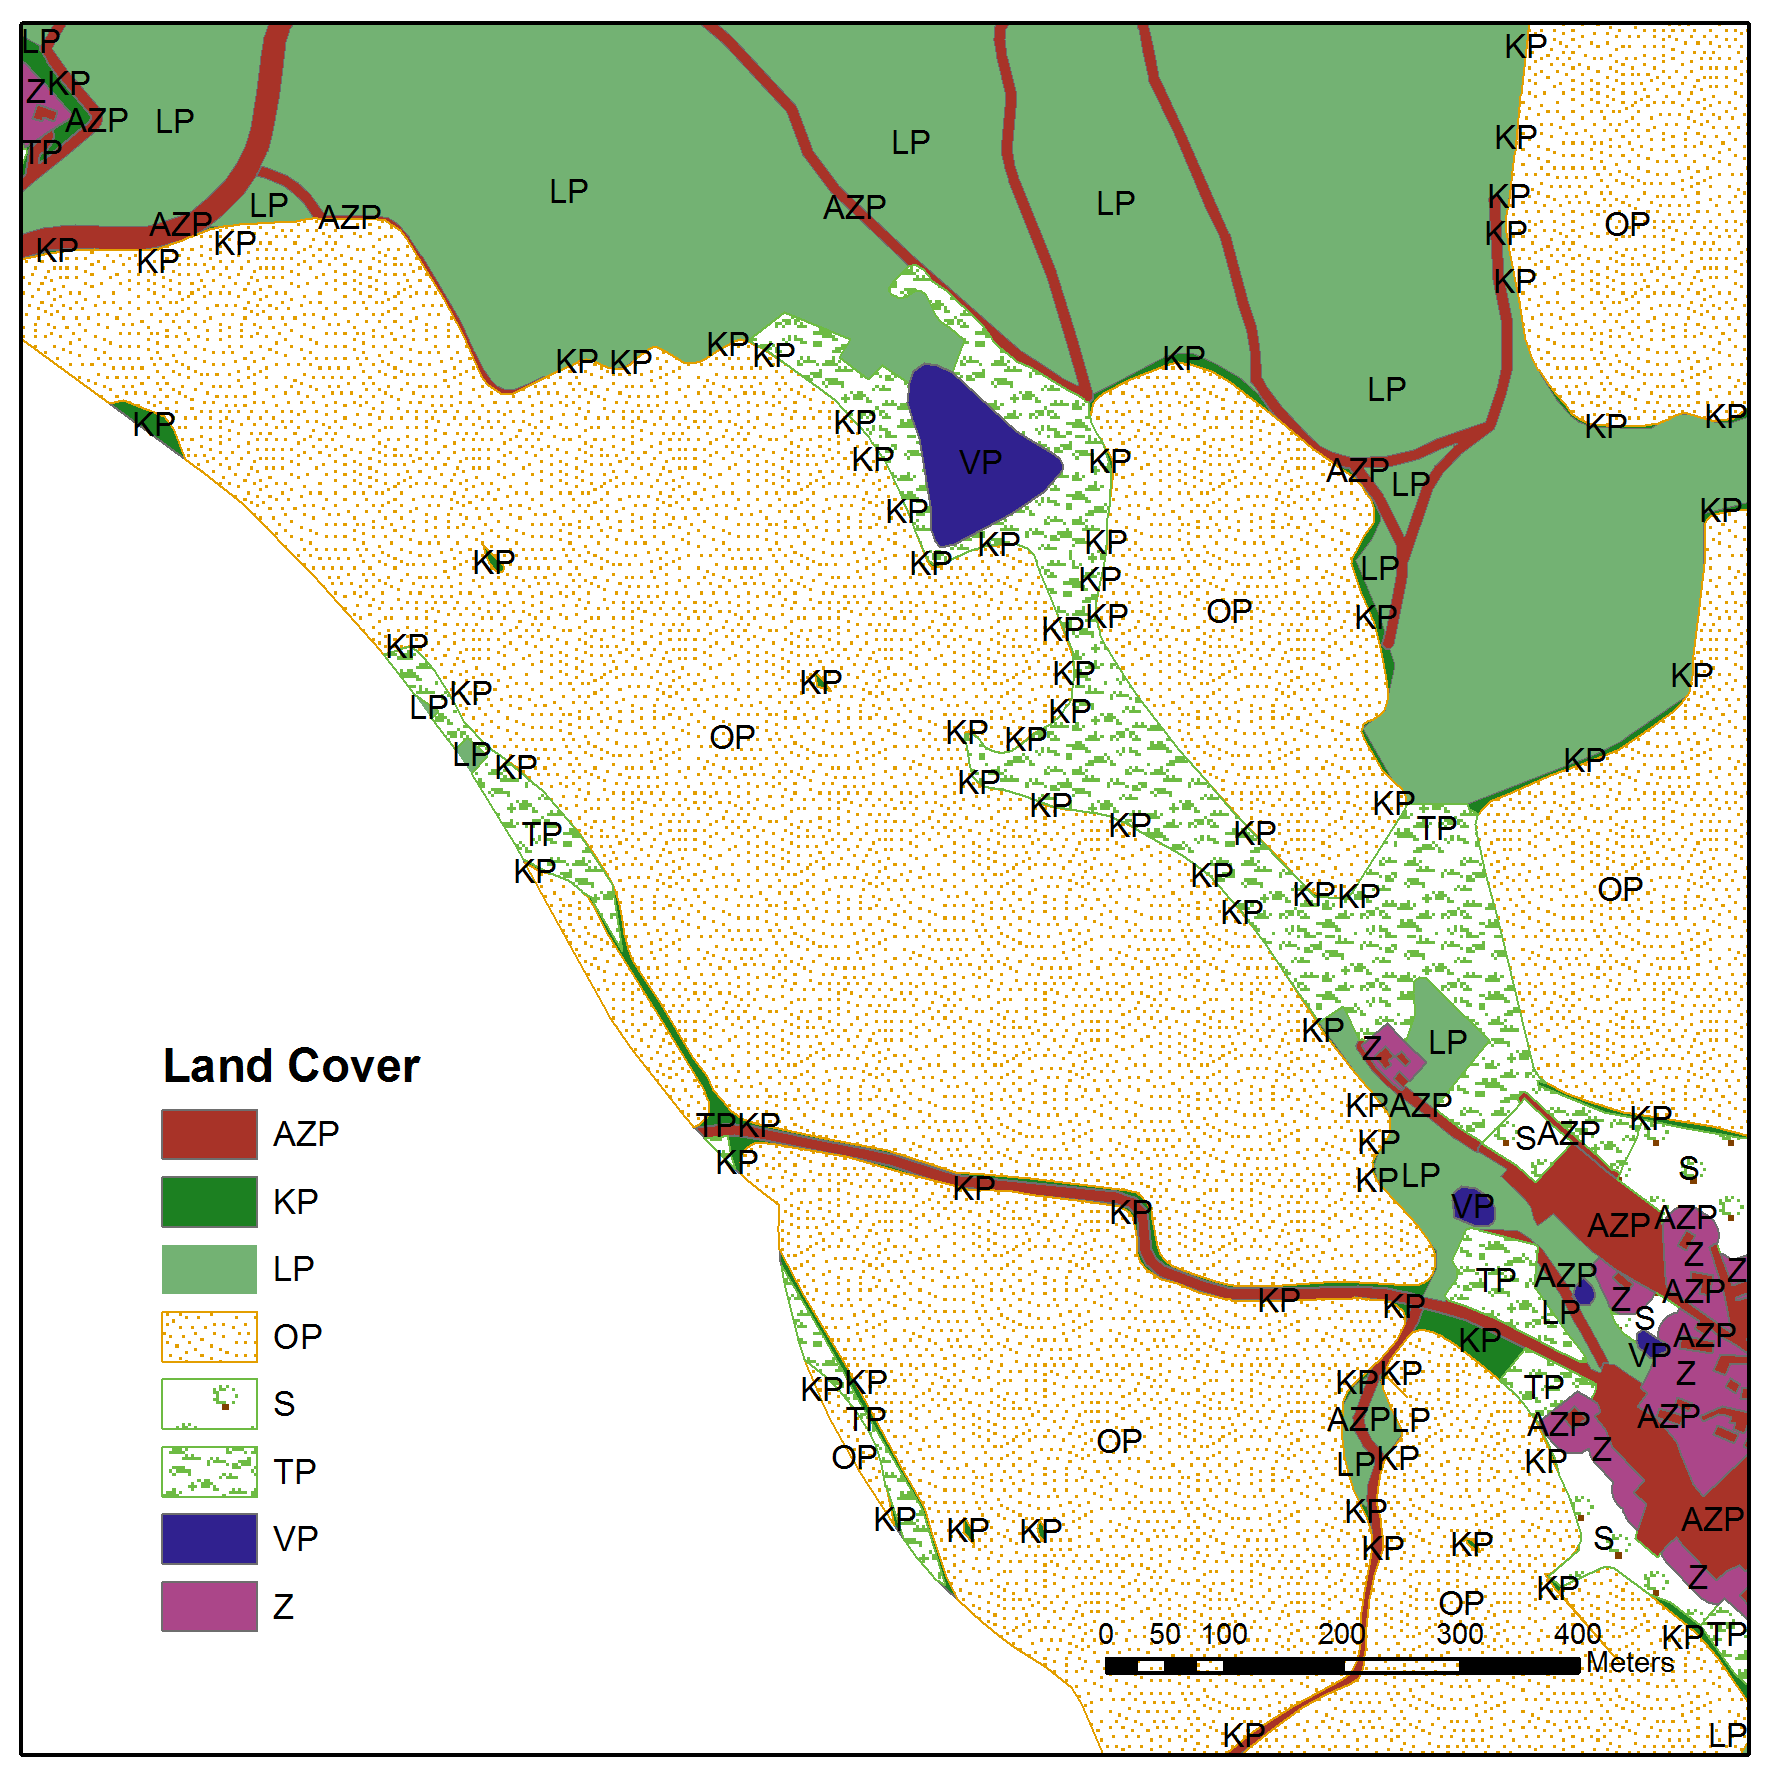
\includegraphics[width=0.5\textwidth]{./img/LandCover.png}
%   \caption{Ukázka vektorové vrstvy využití území -  Land Cover}
%   \label{fig:bykovicevegetace}
% \end{figure}
% 
% 
% 















\subsection{Tabulka parametrů půdy a využití území}  \label{sec:upravatabulkyparametru}

Další povinný vstup je tabulka, která obsahuje hodnoty jednotlivých parametrů popsaných v předešlých kapitolách a v části~\ref{cast:1} toho manuálu. Na tuto tabulku se odkazují identifikátory půdního typu a typu využití území definované pro jednotlivé polygony v atributových tabulkách vektorových vstupů. Tato tabulka může být do modelu vložena jako textový soubor. Na obrázku~\ref{fig:soilvegtablo} je ukázán příklad takové tabulky. V prvních dvou sloupcích jsou identifikátory ($id$) typu půd ($Soil$) a typu využití území ($Land$ $Co.$). Spojením těchto dvou $id$ jsou označeny parametry pro danou kombinaci typu půdy a využití území (třetí sloupec v tabulce na obrázku~\ref{fig:soilvegtablo} s označením $soilveg$). Toto $id$ je pak spojeno s vektorovou vrstvou na obrázku~\ref{fig:prunik}, kde jsou spojeny $id$ z průniku vektorových vrstev půdy~\ref{fig:puda} a využití území~\ref{fig:LU}. Tyto prostorově distribuované parametry jsou následně pro potřeby výpočtu uloženy do rastrů. Hodnoty jednotlivých parametrů pro různé půdní textury, které lze při výpočtu použít, jsou ukázány v tabulce~\ref{tab:kriticke} v příloze~\ref{sec:priloha}. Hodnoty parametrů mají určitý rozptyl, proto se důrazně doporučuje provést jejich měření pro půdy na daném specifickém území.

Význam jednotlivých veličin je popsán v tabulce~\ref{tab:soilveg}. Při přípravě dat je nutné dodržet označení parametrů v této tabulce!




\begin{figure}[t!]
  \centering

  \begin{subfigure}[b]{0.4\linewidth}
    \centering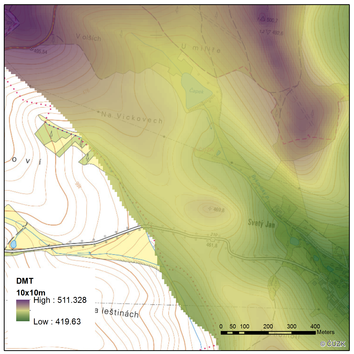
\includegraphics[width=1\linewidth]{./img/DMT_byk.png}
    \caption{\label{fig:dmt}}
  \end{subfigure}%
  \begin{subfigure}[b]{0.4\linewidth}
    \centering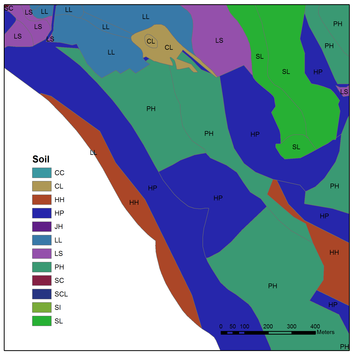
\includegraphics[width=1\linewidth]{./img/pudy.png}
    \caption{\label{fig:puda}}
  \end{subfigure}\\
  \begin{subfigure}[b]{0.4\linewidth}
    \centering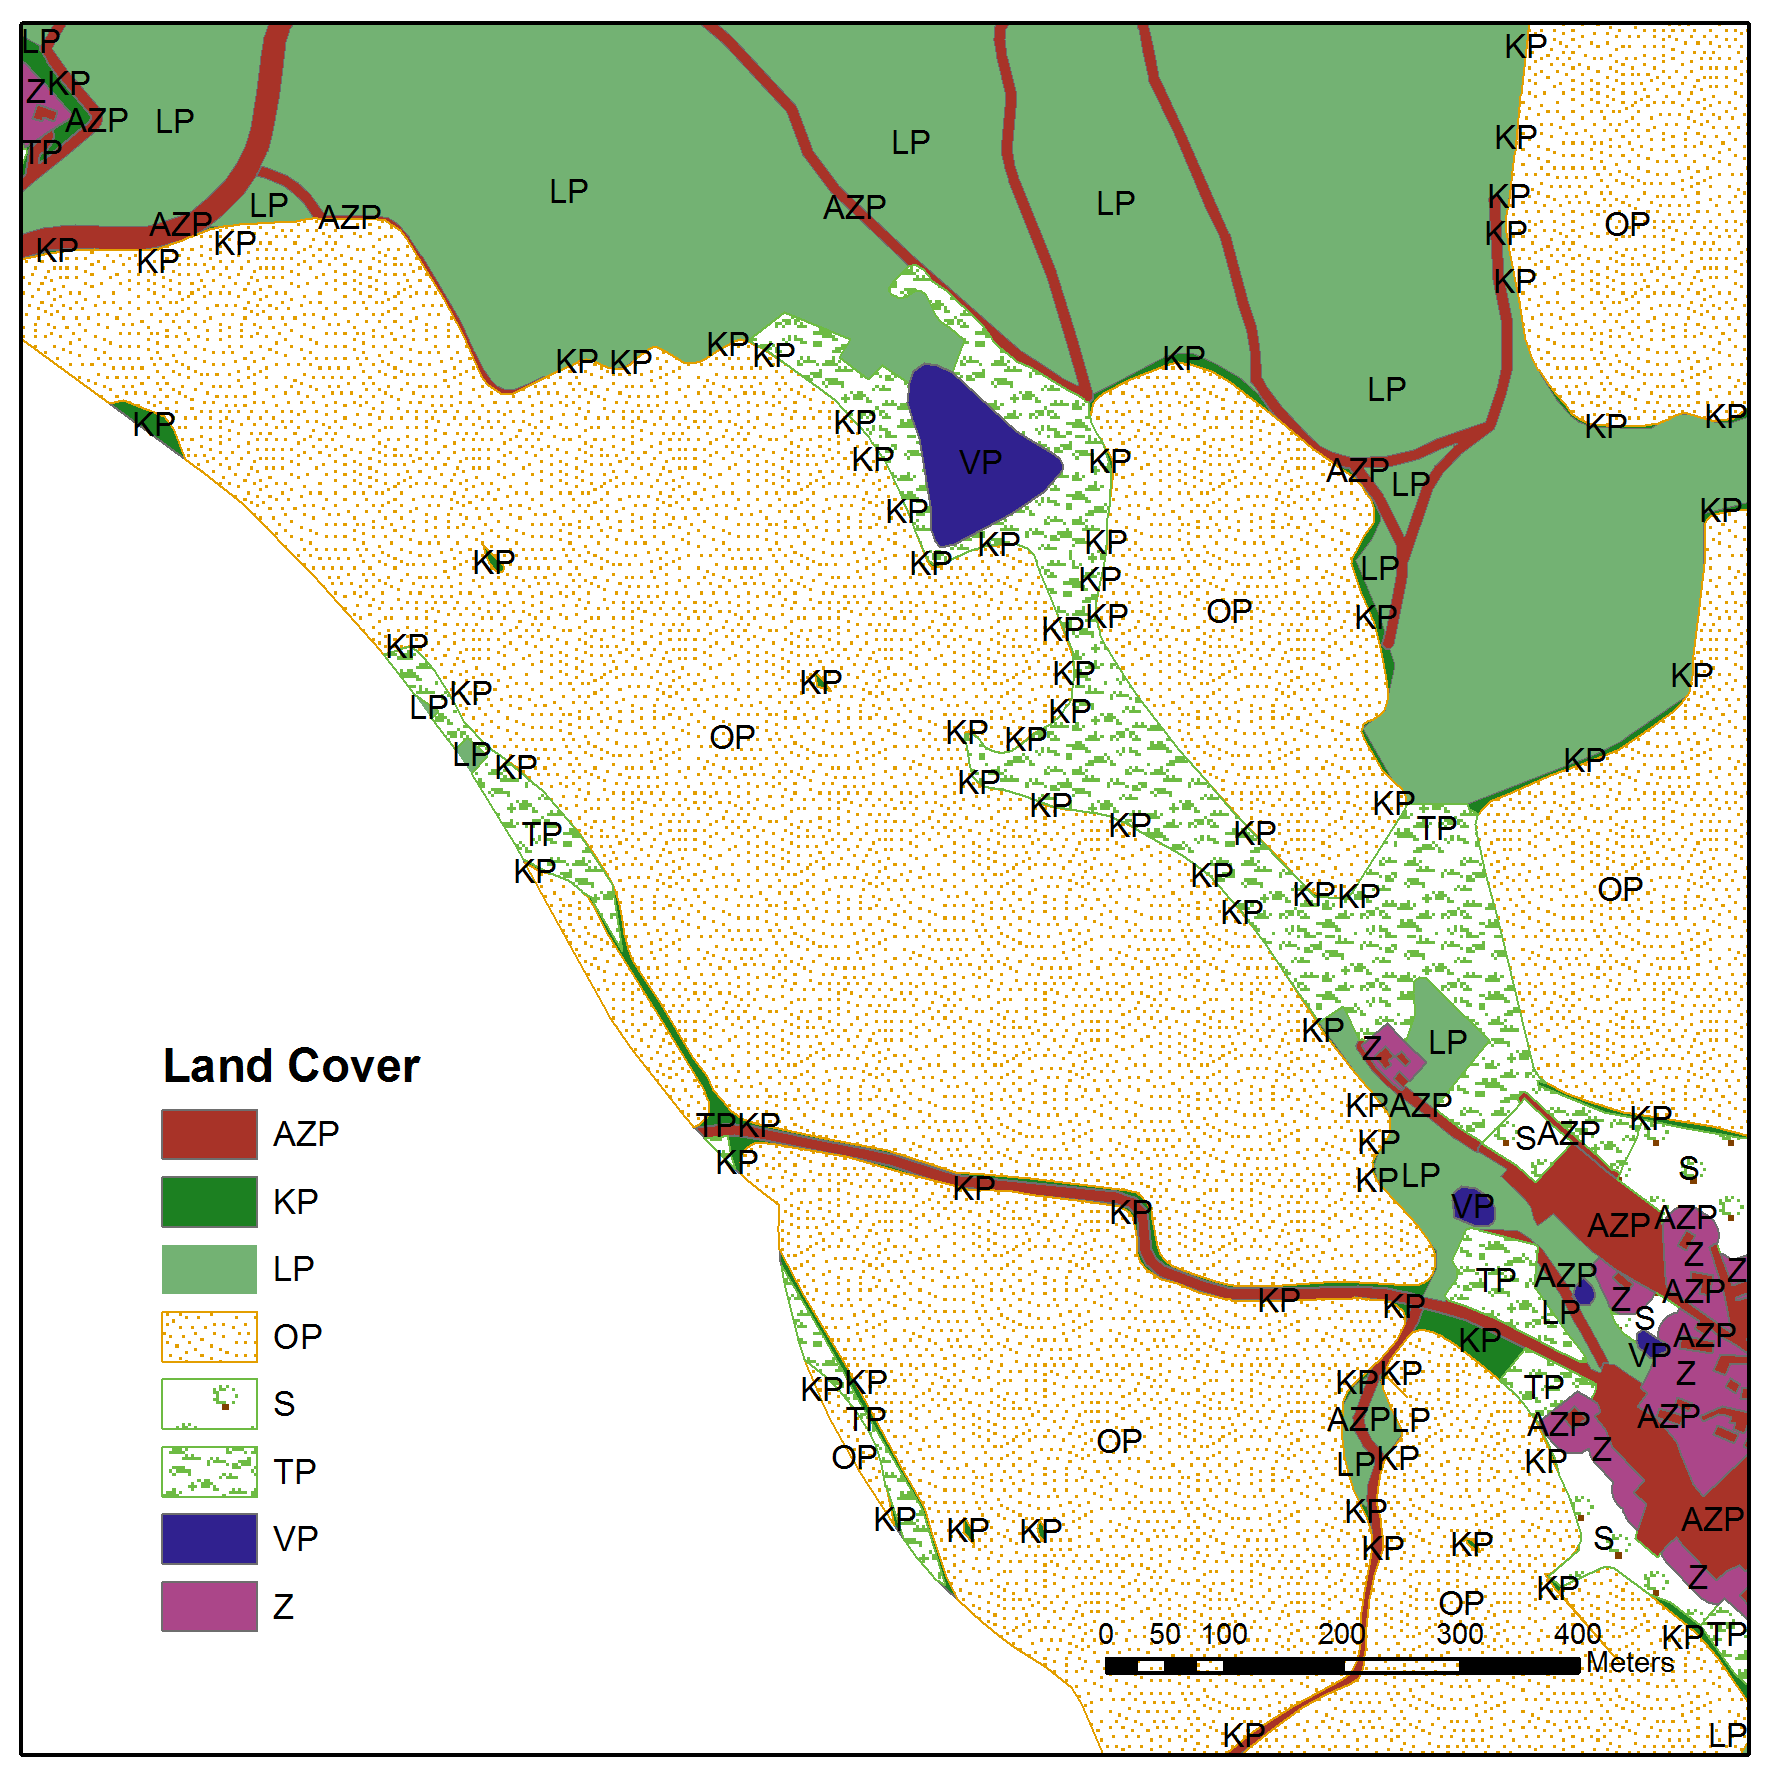
\includegraphics[width=1\linewidth]{./img/LandCover.png}
    \caption{\label{fig:LU}}
  \end{subfigure}%
  \begin{subfigure}[b]{0.4\linewidth}
    \centering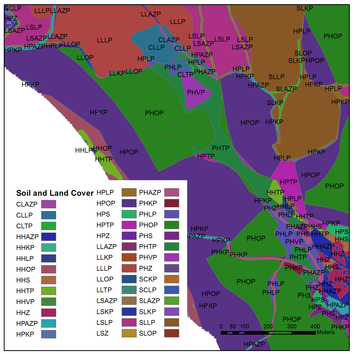
\includegraphics[width=1\linewidth]{./img/SoilAndLC.png}
    \caption{\label{fig:prunik}}
  \end{subfigure}\\
  \begin{subfigure}[b]{0.8\linewidth}
    \centering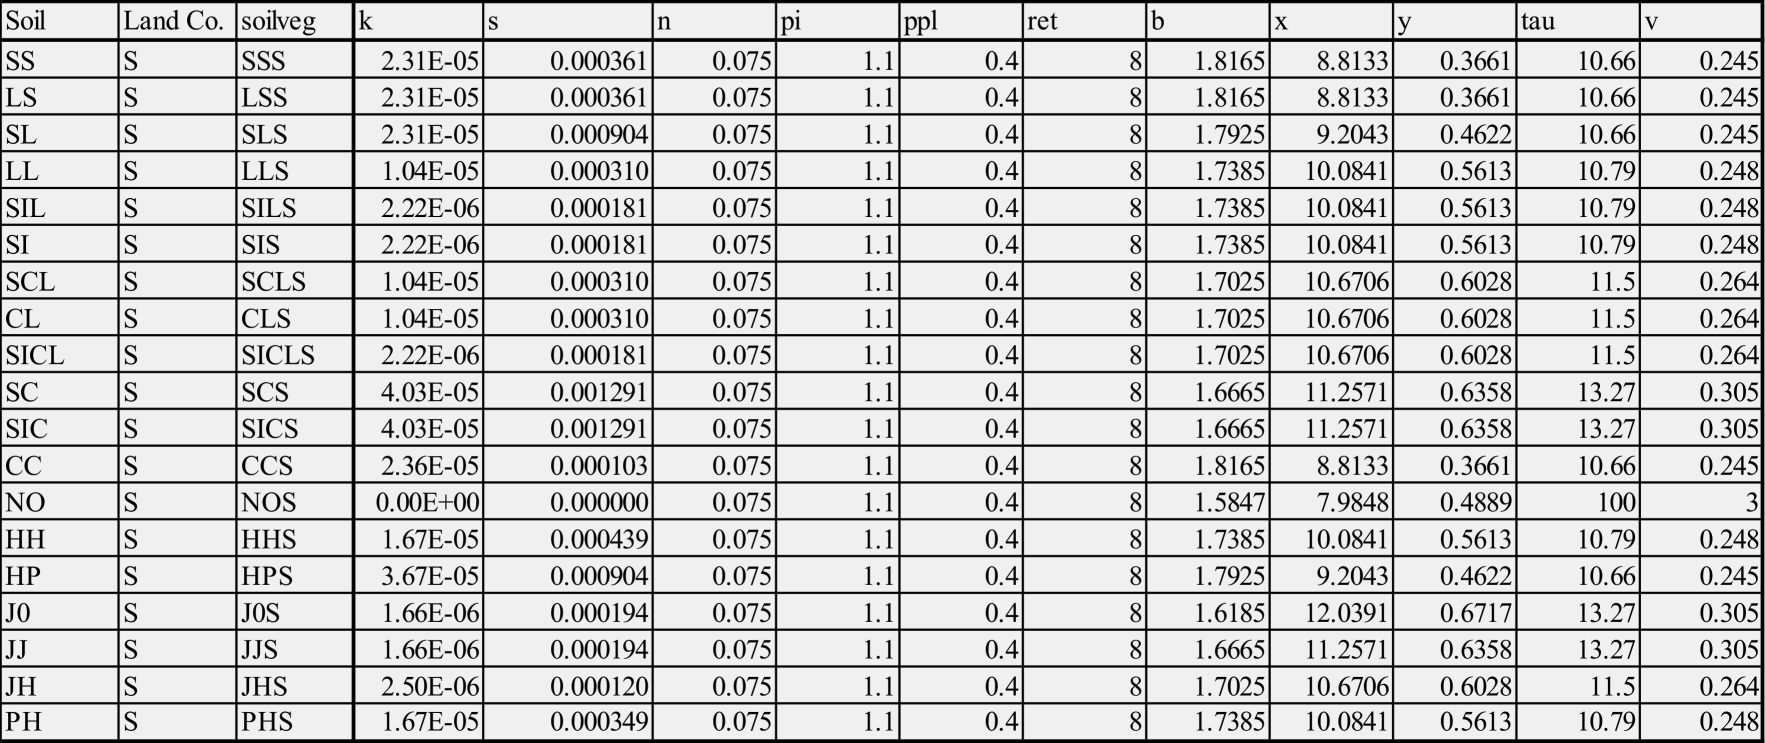
\includegraphics[width=1\linewidth]{./img/soilvegtablo.png}
    \caption{\label{fig:soilvegtablo}}
  \end{subfigure}%
  \caption{Princip propojení vektorových vrstev s tabulkou obsahující parametry typu půd a využití území. Na obrázku a) je digitální model terénu a podkladová mapa. Na obrázku b) je rozložení typu půdy a na obrázku c) rozložení typu využití území. Tyto 2 vrstvy jsou protnuty (funkcí $intersect$). Nové polygony převezmou označení z původních vrstev na obrázku b) a c). Tato nová vektorová vrstva je ukázána na obrázku d). Pomocí převzatých označení polygonů jsou k nim přiřazeny parametry typu půd a využití území z tabulky e).}
  \label{fig:soillu}
\end{figure}



\begin{table}%[!htp]
  \centering
    \caption{Overview of soil type and land use parameters}
    \begin{tabular}{p{3.8cm}l}
    \hline  \hline
        symbol in input table (format mandatory) & description of parameter and unit \\
    \hline
        k&  soil hydraulic conductivity [m/s]\\
        s&  soil sorptivity [$\mathrm{m/s^{1/2}}$]\\
        n&   Mannings surface roughness for sheet flow[-] \\
        b&   power law parameter [-] \\
        y&   power law parameter [-] \\
        nrill&  Mannings surface roughness for rill flow[-] \\
        pi&   potential interception [m]\\
        ppl& canopy cover [-] \\
        ret& surface retention [m] \\
        tau& critical sheer stress [Pa] \\
        v &  critical water velocity [m/s] \\
    \hline  \hline
    \end{tabular}%
  \label{tab:soilveg}%
\end{table}%























\subsection{Srážková data} \label{sec:vstupsrazka}

Dalším vstupem je soubor obsahující srážková data. 
% 
% Na obrázku níže je ukázka textového souboru obsahující proměnlivou srážku, konkrétně je to měření na~rastru Býkovic ze~dne 8.2.2010.
%\begin{figure}[hbt]
%  \centering
 % \includegraphics[scale=1]{obrazky/srazkovysoubor.png}
  %\caption{Srážkový soubor}
%  \label{fig:srazkovysoubor}
%\end{figure}
% 
% 
Srážky se zadávají jako textový soubor se dvěma sloupci. V levém sloupci je časový interval v minutách, v pravém sloupci je \textbf{kumulativní úhrn} za daný časový interval v \textbf{milimetrech}. Ukázka jednoduché srážky a grafické reprezentace kumulativních dat je na obrázku~\ref{fig:srazkovysoubor}. První záznam vyjadřuje srážku od času 0 do například 10 minut (obrázek~\ref{fig:srazkovysoubor}). První záznam v textovém souboru musí mít nenulový čas i úhrn. Soubor může obsahovat prázdné řádky, které jsou ignorovány, nebo komentáře začínající \#. 
\begin{figure}
  \centering
  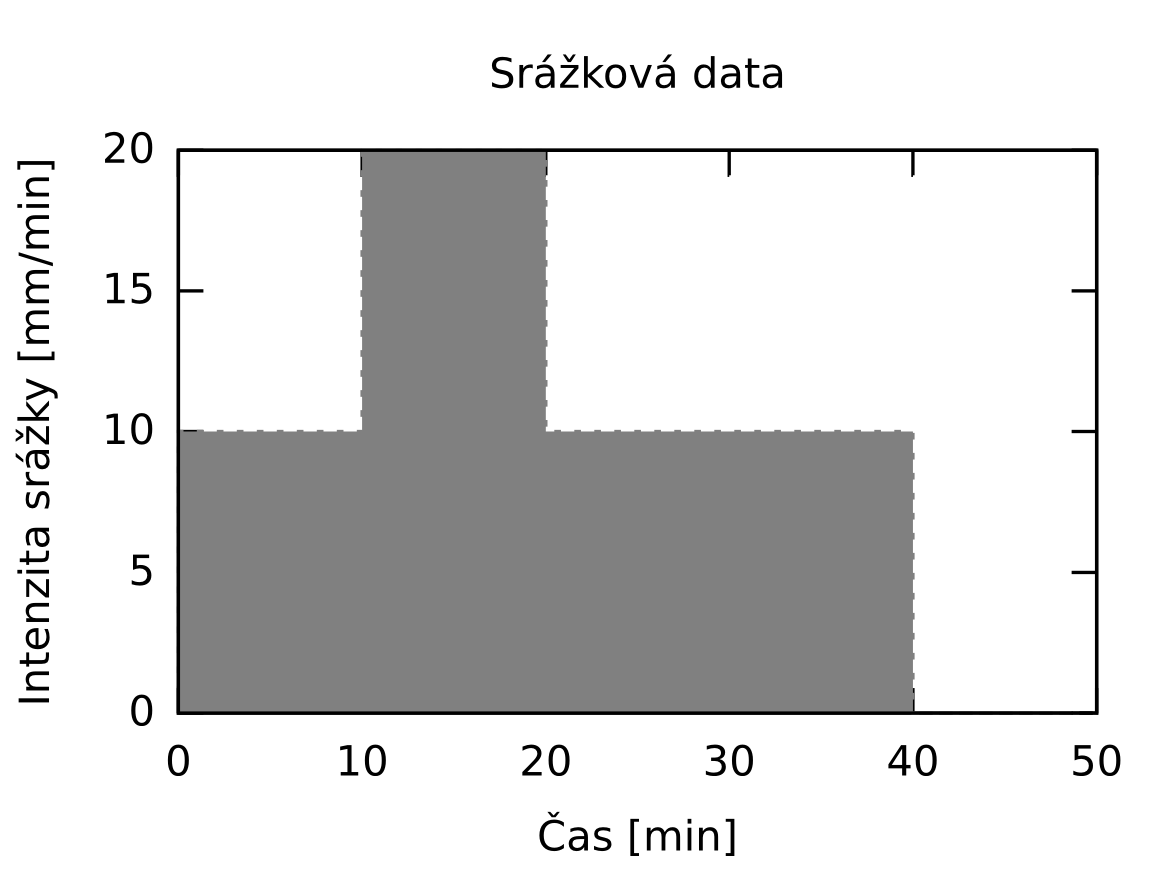
\includegraphics[width=0.45\textwidth]{./img/srazka-graf.png}
  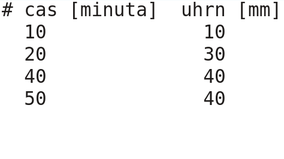
\includegraphics[width=0.5\textwidth]{./img/srazka-soubor.png}
  \caption{Ukázka srážkových dat. Vlevo: grafická reprezentace zadaných dat (srážka zobrazena v intenzitách; Napravo: ukázka dat v požadovaném formátu).}
  \label{fig:srazkovysoubor}
\end{figure}














\subsection{Časový krok modelu a celková doba výpočtu} \label{sec:vstupkrok}

Časový krok modelu \acs{dT} je hodnota v sekundách. Jako vstupní parametr se zadává maximální časový krok. Tento časový krok je rovněž počáteční časový krok. Časový krok \acs{dT} je v průběhu výpočtu upravován podle Courant-Friedrich-Lewy (\acs{CFL}) podmínky tak, aby byla zachována numerická stabilita. Délka časového kroku závisí na rychlosti povrchového odtoku a na velikosti prostorového kroku (velikosti buňky DMT). Maximální časový krok záleží na požadovaném detailu výstupních dat, zejména při dotoku srážkové epizody, kdy jsou již rychlosti proudění nižší a kdy by \acs{CFL} kritérium povolovalo příliš velký časový krok. Zvolené řešení změn časového kroku je detailněji popsáno v kapitole \ref{sec:cfl}. 

%Vzhledem k tomu, že rychlost odtoku v rýhám může být řádově vyšší než rychlost plošného odtoku je snaha řídit velikost časového kroku podle rychlosti plošného odtoku, kde Courantovo kritérium povoluje vyšší časový krok. Velikosti časového kroku zásadně ovlivňuje celkovou délku výpočtu. Pokud časový krok vyhovuje Courantovu kritériu v plošném odtoku, ale toku v rýhách již nikoli, začne se časový krok dělit pouze interně při výpočtu rýh. Tyto děje se probíhají při běhu programu a uživatel je nijak neovlivňuje, nicméně, je třeba si uvědomit, že při vytvoření rýhového odtoku a nutností dělit časový krok v těchto buňkách může se doba výpočtu jednoho časového kroku prodloužit. která udává velikost jednoho kroku výpočtu, v němž probíhá výpočet odtoku a další nedílné součásti programu. Zadaný časový krok se mění podle potřeb Courantova kritéria \ref{section:cfl}, nikdy však nemůže být vyšší než vstupní zadaná hodnota uživatelem. 

%Při zadávání počátečního časového kroku je možno zvolit hodnotu v rozmezí od 0.05 do 0.3 minuty. 
% Velikost časového kroku nejvíce ovlivňuje reálnou dobu běhu modelu. Čím nižší je časový krok, tím déle uživatel čeká na výsledky. 
%Stejně jako u všech ostatních číselných hodnot zadávaných do programu ArcGIS je potřeba myslet na to, že čísla s desetinnými místy musí být odděleny tečkou, nikoliv čárkou.

Konečný čas simulace je hodnota v minutách. Délka běhu modelu by měla být taková, aby odtekla veškerá voda z řešeného území, především při zjišťování celkového objemu odtoku.
 


%\subsection{Povrchová retence} \label{sec:vstupretence}

%Povrchová retence je děj, při kterém se zachytává počáteční část srážky, která se dále neúčastní odtoku. V reálném prostředí si lze toto představit jako zachytávání srážkové vody v nerovnostech na povrchu. Pouze po naplnění těchto malých nerovností dochází k povrchovému odtoku. Hodnota závisí na hustotě půdy a její deformaci. Povrchová retence se zadává v mm. Pro veškerá testování byla povrchová retence zvolena 0.2 mm.













\subsection{Body pro generování hydrogramů} \label{sec:vstupbody}

Jedná  se o volitelnou bodovou vektorovou vrstvu. V těchto bodech se budou ukládat časové řady počítaných veličin (hydrogramy). Obsah časových řad je podrobněji popsán v kapitole~\ref{sec:hydrogramy}.











\subsection{Výstupní adresář} \label{sec:vstupadresar}
Do výstupního adresáře se uloží veškeré výstupy modelu. Na začátku běhu programu se obsah tohoto adresáře celý vymaže, proto se doporučuje vždy provést kontrolu. V žádném případě nenastavujete jako výstupní adresář pracovní plochu, či jiný adresář, kde byste mohli mít uložená důležitá data!

% % % % \subsection{Rýhový odtok} \label{sec:vstupryhovy}
% % % % Tento volitelný parametr po zaškrnutí umožní výpočet soustředěného odtoku. Soustředěný odtok je popsán v sekci \ref{sec:soustredenyodtok}.










% 
% \subsection{Vícesměrný odtok} \label{sec:vstupvicesmerny}
% 
% Výchozí odtokový algoritmus \acl{D8} \acs{D8}. Parametr volby vícesměrného odtokového algoritmu je volitelný. Více o tomto typu odtoku je v části \ref{subsection:MD}
% 
% 
% 







\subsection{Hydrografická síť} \label{sec:vodnitoky}

Hydrografickou sítí jsou myšleny nejen vodní toky, ale i prvky dočasné hydrografické sítě jako jsou příkopy, průlehy, cesty s příkopy a pod. Výpočet v modelu probíhá po jednotlivých úsecích pomocí Manningovy rovnice pro výpočet průtoku (popsané v části~\ref{cast:1}). Prostorové umístění jednotlivých úseků je definované pomocí shapefile liniové vrstvy. Charakteristiky jednotlivých úseků jsou definovány v samostatné tabulce. Pro propojení prostorové informace s charakteristikami úseků je třeba mít v této tabulce shodný název pole jako ve vrstvě vodních toků, kde jsou uloženy označení jednotlivých typů příčných profilů.

V tabulce~\ref{tab:toktab} je ukázka zadávaných hodnot.  Model umožňuje vybrat ze čtyř tvarů příčného průřezu úseků, kde každý tvar má povinné celočíselné označení. Tyto tvary jsou: obdélník (výchozí; tvar: 0), lichoběžník (tvar: 1), trojúhelník (tvar: 2) a parabola (tvar: 3). Kromě tvarových charakteristik (šířka dna, sklon břehu) lze rovněž definovat základní průtok ve formě 365-ti denního průtoku. Pokud úsek charakterizuje objekt, který je pouze dočasně zavodněný, je Q365 = 0. Pole, které slouží k připojení parametrů z tabulky k jednotlivým úsekům hydrografické sítě je v tabulce~\ref{tab:toktab} označeno jako $smoderp$. Rovnice použity při určení hydraulického poloměru jednotlivých tvarů příčných profilů jsou ukázány v tabulce~\ref{fig:tvary_koryt} v příloze~\ref{sec:priloha}.
% 
% Zadávání tvaru příčného profilu není součástí atributové tabulky shapefile, ale pro ulehčení jsou parametry zadávány v samostatná tabulce. V případě, že jsou některé charakteristiky shodné, je tak možné jim přiřadit shodné atributy z tabulky.
% V rámci zjednodušení výpočtu jsou zadávány profily parametricky. Zjednodušený výpočetní model neuvažuje rozlivy z koryta zpět do buněk odtoku. Jednotlivé prvky narůstají podle zvolených parametrů, tak aby veškerá voda zůstala v korytě.
% přehled parametrů je uveden v tabulce~\ref{tab:toptab}

\begin{table}[htb!]
\centering
\caption{Příklad tabulky s parametry jednotlivých úseků hydrografické sítě}
\label{tab:toktab}
\begin{tabular}{llcccccc}
\hline
% 
cislo & smoderp      & tvar & b   & m   & n & Q365 & pozn           \\ \hline \hline
0      & 0            & 1    & 0.3 & 1.0 & 0.03    & 0.0  & default \\
1      & obdelnik1    & 0    & 0.2 & 0.0 & 0.035   & 0.0  &         \\
2      & lichobeznik1 & 1    & 0.2 & 2.0 & 0.035   & 0.0  &         \\
3      & trojuhelnik1 & 2    & 0   & 2.0 & 0.03    & 0.0  &         \\
3      & trojuhelnik2 & 2    & 0   & 2.5 & 0.03    & 15.0  &        \\
4      & parabola1    & 3    & 0.7 & 0.0 & 0.03    & 0.0  &         \\ \hline
\end{tabular}
\end{table}
\FloatBarrier
% 
% 
\begin{tabular}{rrl}
   kde \jj{bhs}{,}
       \jj{m}{,}
       \jj{n}{\ a}
       \jj{Q365}{.}
%        \jj{Rstream}{.}
\end{tabular}

% 
% \pozn{
% kde:
% \begin{itemize}
% \item \textbf{b} - šířka profilu ve dně (u trojúhelníku se rovná nule)
% \item \textbf{m} - poměr sklonu svahů (pro obdélník je roven nule)
% \item \textbf{drsnost} - Maninngova drsnost v daném korytě.
% \item \textbf{Q365} - základní odtok. V případě dočasných prvků jako jsou příkopy je tato hodnota rovna nule, v případě vodních toků se jedná o základní odtok.-
% \item \textbf{poznámky} - jedná se o volitelnou položku, do výpočtu se nijak nepropaguje
% \end{itemize}
% }
% 
% 
% 

